
\chapter[Visual Cue Based Corrective Feedback for Motor Skill Training in Mixed Reality]{Visual Cue Based Corrective Feedback for Motor Skill Training in Mixed Reality: A Survey\label{chap:visualCueSurvey}}

Physical activity, especially exercise and physiotherapy, is important to improve and retain a healthy condition. In recent years, instructions and feedback given to learn and execute the relevant body movements have been increasingly supported by technology. In particular, systems employing \acrfull{mr} and \acrshort{ar} have been devised to support this so-called \emph{motor skill training}. The \acrshort{vr} and \acrshort{ar} technologies represent a platform for innovative new visualization techniques regarding motor skill training which are worth exploring.

In this chapter, we survey such approaches of visual feedback using \acrshort{vr} in the field of physical therapy, exercise and motor skill learning in general regarding the different visual feedback and technologies involved. In comparison to the existing surveys (see \autoref{sec:relatedwork}), we look deeper into which visual cues are used and how they are employed to achieve the goal of movement correction. To achieve this aim, we devise a classification of the approaches surveyed which involves, among other aspects, the used \acrshort{vr} technologies, temporal and spatial characteristics of the feedback given, and the body parts addressed by the feedback. Additionally, we relate the approaches to stages of the way humans learn skills~\cite{fitts1967HPe}. The intention is to obtain a clearer view of which visualization techniques and visual cues are suitable for given tasks and to show where there are gaps in the existing research. The former can help practitioners and developers choose the appropriate visual cues for their task and system, while the latter can show researchers avenues for future research. 

This survey discusses approaches from 39 papers which were selected
out of 131 papers initially reviewed. These approaches were found to be relevant in terms of providing insight into the types of corrective visual motion feedback investigated in current research.

The focus of our analysis is aimed at the visual feedback of the surveyed literature. This does not include the therapeutic and medical aspects. We listed surveys addressing these points in \autoref{sec:relatedwork}.

\begin{figure*}[tb]
    \centering
    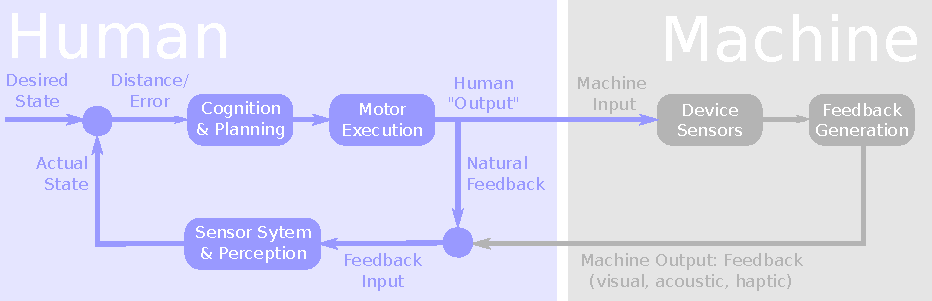
\includegraphics[width=1\linewidth]{pictures/feedbackloop.pdf}
    \caption[Illustration of the human-machine feedback loop based on~\cite{morone2021dab}\label{fig:feedback}.]{Illustration of the human-machine feedback loop based on~\cite{morone2021dab}\label{fig:feedback}. The \emph{machine} or \emph{system} usually is a computer with some kind of display, for example an \acrshort{ar} headset.}
\end{figure*}

\subsection{Related Work\label{sec:relatedwork}}
There is a limited number of surveys discussing visual feedback in \acrshort{vr}. While their scope regarding use cases, body parts, or technologies is often narrower than ours, the analysis regarding the types of feedback and the forms it can take is broader. The survey at hand goes in more depth regarding feedback while retaining a wide scope of use cases, body parts, and technologies. In the following paragraph, we will discuss related surveys and ways in which our work complements the existing research.

The scope of the present work, and therefore the scope of the related surveys, is located at an intersection between medicine, sports, and computer science. In the medical literature, surveys like Mubin et al.~\cite{mubin2020esg}, Schiza et al.~\cite{schiza2019vra}, Gandhi et al.~\cite{gandhi2020mts} and Rutowski et al.~\cite{rutkowski2020uvr} provide a treatment-oriented perspective on the field of digital feedback for movements. Their overview and analysis are mainly focused on the outcome of the treatment and less so on the type of visual feedback. The chapter at hand however is concerned with the visualization of the feedback given. Related surveys from the \emph{physical exercise} part of the literature, in particular, Perin et al.~\cite{perin2018sas} and Liebermann et al.~\cite{liebermann2002aai}, look at the performance regarding exercise.
One topic connected to visual feedback is (serious) gaming. Thus, it is worth noting that the above-mentioned Mubin et al. \cite{mubin2020esg} and Ma et al.~\cite{ma2011vrp} discuss serious games in health care. Sawan et al.~\cite{Sawan2016MRS} present a literature review on how various \acrshort{vr} and \acrshort{ar} technologies are used in the sports industry. The review provides insights on the sport-related use cases of \acrshort{vr} and \acrshort{ar} technologies.

Gatullo et al.\cite{gatullo2020whw} conducted a systematic literature review and classification for visual assets in industrial \acrshort{ar} applications. As skill learning and training are an important use case for \acrshort{ar} in the industrial context, their work is related to ours. The focus of their approach, however, lies heavily on tool handling, which we excluded from the scope of this work (see~\autoref{sec:tvcg:methodology}).

In addition to these generally related publications, there are a few papers that stand out as being closer to our approach, as they analyze visual aspects of feedback and hence have a scope overlapping ours:

Viglialoro et al.~\cite{viglialoro2019rar} investigate literature aiming at \emph{shoulder rehabilitation} supported by \acrshort{ar}. The scope of their review led to a sample collection of nine papers. The arm and hand movements of the users, as well as rehab settings, target groups, tracking technologies of each \acrshort{ar} system, user interfaces, and evaluation methods, were investigated.

The work of Neumann et al.~\cite{neumann2018sra} surveys 20 approaches focusing on \emph {\acrfull{vr}} in physical exercise. They investigated activity, equipment, \acrshort{vr} technology, \acrshort{pov}, and whether other persons than the user are present in the environment. The characteristics of test groups were looked at as well. The number of participants, gender, age range, experience type, and location were investigated and documented. Additionally, the paper summarized the aims, conditions, measured features, immersion, and key findings of the researched literature.

Brennan et al.~\cite{brennan2019fdt} analyzed literature about feedback design in \emph{home rehabilitation}. While this comes close to our approach, they did not focus on MR and limited their scope to home rehabilitation, which resulted in a smaller body of literature of only 19 research attempts. Clinical context, system components, feedback design, and the evaluation of these features were investigated. The feedback characteristics were categorized and analyzed. This resembles our approach, although we took a closer look at the visualizations \emph{per se}. The smaller scope of our survey in comparison to the approach of Brennan et~al. enabled us to analyze visual cues in more detail.


\subsection{Organization of this Chapter}
This chapter starts with an introduction establishing the motivation of the present survey and relating it to previous works as well as putting it in scientific context. Relevant terminology and fundamental concepts like feedback and skill learning basics are introduced in \autoref{sec:background}. In \autoref{sec:tvcg:methodology} our methodological approach to acquiring literature is explained and the guidelines we followed to do so are described. \autoref{sec:classification} elaborates on how we categorized the literature and the features we chose for that matter. \autoref{table:2} shows the results of our classification and represents a central point of reference for the whole chapter. To make the nature of the surveyed literature more accessible to the reader, an exemplary discussion can be found in \autoref{sec:exemplary}. In \autoref{sec:tvcg:insights} the main insights of this survey are presented. The chapter is concluded by summarizing the findings, mentioning limitations, and highlighting interesting open questions in \autoref{sec:tvcg:conclusion}.


\section{Background and Terminology \label{sec:background}}
To establish a common ground for understanding and discussion, we explain the definitions of the most important terms in this section. Additionally, we provide an overview of the fundamental concepts we are working on in this chapter.

\subsection{Feedback \label{sec:feedback}}
The term \emph{feedback} originates from electronics as stated by Morone et al. \cite{morone2021dab}. In this context, the output of a system is combined with the input to affect the function of the system. This idea was later transferred to the social sciences, as humans observe their \emph{actual state} and regulate their behavior according to a \emph{desired state} to minimize an \emph{error} (or \emph{distance} in our case), as stated by Morone et al.~\cite{morone2021dab}. This idea is illustrated in \autoref{fig:feedback}. The \emph{natural feedback} loop, which is represented on the left in \autoref{fig:feedback}, involves planning, executing, perceiving, and adjusting the movement.


This feedback loop can be extended to incorporate a technical feedback system as seen in the literature we analyze (represented by the right loop in \autoref{fig:feedback}). To provide feedback, the machine detects certain aspects of the human output (in our case the movement). This information then enters the system as \emph{machine input} via \emph{device sensors}. The machine-\emph{generated feedback} is then delivered to the human as a (in our case visual) \emph{machine output}.

The scope of the present chapter includes literature which for the most part includes what Morone et al.~\cite{morone2021dab} define as 'augmented feedback'. This means the user is already aware of the feedback signal given by the system. In our case, the visual information of the body position in space is emphasized by the feedback, and a focus is placed on movements that the users can readily detect themselves.

The term \emph{augmented feedback} has to be distinguished from the term \emph{biofeedback}, which is commonly used in current literature. It often occurs in the context of device-supported rehabilitation feedback. When used accordingly, it refers only to signals the users are not aware of, for example in electromyography (EMG), where the electrical activity of the muscle is measured \cite{mills2005bem}.

In educational settings, feedback is traditionally given by another person, usually a teacher, instructor, or trainer (see \autoref{sec:instructor}). In this context, feedback that enables participants to correct their behavior is often called \emph{corrective feedback}~\cite{hattie:2007:Feedback,Lysakowski:1982:Feedback}. Similarly, in a feedback system, information qualifies as corrective feedback if it gives the user insight into how the movement can be carried out differently in order to accomplish the task at hand correctly or at least in an improved manner. 

To be precise at this point, it has to be mentioned that in computer science 'feedback' is often used for the response of a system to confirm input by the user~\cite{ADictionaryofComputerScience}. This meaning of the term is not relevant to the scope of this chapter.

\subsection{Phases of Skill Learning in Physical Activity\label{sec:stages}}
The acquisition of new skills proceeds in three stages or phases as described by Fitts and Posner~\cite{fitts1967HPe}. These phases of skill learning are connected to motor skill acquirement as shown by various authors (see e.g. \cite{schmidt2004motor,SWINNEN1997749,SINGER197879} and \cite{taylor2012rsm}). The three stages as seen in \autoref{table:1} successively take place one after another over the course of internalizing a movement.

Skill acquisition starts in the \emph{cognitive} stage, where the learner tries to grasp the overall concept and understand what to do. The flow of information from an instructor (or instructions) to the learner plays a major role during this phase, as the learner still processes what to do. 
In the \emph{associative} stage the learner will construct the actions to be done from minor movements (subroutines) and the information gathered during the cognitive stage.
The final stage is the \emph{autonomous} stage. Herein the learner has fully internalized the movement. The cognitive capacity needed for the movement is minimal in this stage. Thus, additional information can be accessed or processed while making use of the skill. The efficiency and performance of the activity enacted still increase in this stage.

Once the learners have internalized an action, they can revisit stages to improve and 'relearn' their movements~\cite{huber2013AEP}. As stated by Fitts and Posner~\cite{fitts1967HPe} the transitions between stages are not always clear. Nevertheless, it will be useful in the survey at hand to relate the skill level of the target group to the feedback given.

\begin{table}[ht]
\caption[Fitts and Posners stages of skill learning~\cite{fitts1967HPe}.]{Fitts and Posners~\cite{fitts1967HPe} stages of skill learning as applied to motor learning. Presentation based on~\cite{huber2013AEP}.\label{table:1}}
\begin{tabular}{ |p{2.2cm}||p{2.6cm}|p{5.2cm}|p{2.2cm}|  }
    
 \hline
 Stage & Process & Characteristics & Other name\\
 \hline
 \hline
 Cognitive & \raggedright Gathering Information & \raggedright Large gains, inconsistent performance & Verbal-motor stage \\
 \hline
 Associative & \raggedright  Putting actions together & \raggedright Small gains, disjointed performance, conscious effort & Motor stage \\
 \hline
 Autonomous & Much time and practice & Performance seems unconscious, automatic and smooth & Automatic stage \\
 \hline
\end{tabular}
\label{table:stages}
\end{table}

\subsection{Instructor or Agent\label{sec:instructor}}
In Fitts and Posner's work~\cite{fitts1967HPe} discussed above, instructors play a central role. They transfer knowledge to the learner and decide what input is suitable at a given moment. In most \acrshort{vr} systems, a machine substitutes the instructor as illustrated in \autoref{fig:feedback}. This means that feedback systems have to be designed carefully with the user in mind (participatory design)~\cite{davies2003vrf}. Oftentimes health care professionals are included in this process~\cite{hilton2011dem}.

Hattie and Timperley establish the more general notion of an \emph{agent} in their work~\cite{hattie:2007:Feedback}. This notion includes teachers, peers, books, parents, the self, and experience. It can be regarded as analogical to the term instructor. A \acrshort{vr} system substituting the human instructor qualifies as such an agent. Virtual Trainers, virtual medical professionals, and simplified human shapes are depicted in \acrshort{vr} to provide feedback to the user, to hint at positional discrepancies, or to show in advance what positions to copy. A good example for this is the work of Mostajeran et al.\cite{mostajeran2019hvc}, which utilizes a virtual coach offering instructions to the user.

A few systems included in our survey, like those described by Debarba et al.~\cite{debarba2018arv} and Furukawa et al.~\cite{furukawa2018dar}, provide feedback to instructors. These approaches are applied to rehabilitation but could also be applied to physical exercise or skill learning in general. One advantage of systems targeting instructors is the exact metrics they can provide to the instructors. Consequently, the instructor is well-informed and can decide what information to give to the learner or client.

\subsection{Immersion \label{sec:immersion}}
As discussed by Nilsson et al. \cite{Nilsson2016irr}, there are various definitions of immersion that seem to differ from one another quite considerably.
What they all seem to have in common is that immersion influences a feeling of \emph{presence}, an impression of being there. Ijsselsteijn et al. \cite{ijsselsteijn2004fas} established that immersion, and connected with it, presence help to motivate users. They even increase the feeling of competence and control, which is highly relevant when applying a given feedback and hence correcting a false movement.

\section{Methodology and Scope \label{sec:tvcg:methodology}}
To acquire literature for this survey, we conducted \emph{snowballing} as a search approach. The snowballing followed a scheme similar to the one described by Wohlin \cite{wohlin2014gss}. We preferred snowballing rather than database keyword searches because it has been shown to be more effective for acquiring sources in general (see \eg\ Greenhalgh et al. \cite{greenhalgh2005ees}, Badampudi et al. \cite{badampudi2015eus}). As \emph{start set} for the snowballing, we used the papers mentioned in related works (\autoref{sec:relatedwork}). While snowballing, we did not limit ourselves to papers, but included all sources of interest to the research community, considering all sources which incorporate motor skill training in \acrshort{vr}.

To decide which of the papers obtained to include in the survey, we conducted a screening analogical to the flow diagram of the PRISMA (Preferred Reporting Items for Systematic Reviews and Meta-Analyses) guidelines described by Liberati et al. \cite{liberati2009prisma}.

Since the field of \acrshort{vr} is moving fast and there have been major changes and innovations in recent years, we additionally limited the publications to be surveyed to those which have been published in the period since 2016. The year 2016 marks the launch of Microsoft's \acrshort{ar} headset \emph{HoloLens} which represents an important development to the research community in the field of \acrshort{vr} applications~\cite{Park2021}.

In detail, through snowballing with the above-mentioned scope, we identified 131 promising papers. After screening, we found 28 papers were not relevant to our overview, since their keywords or title might have sounded promising, but their content did not match our scope. Subsequently checking for eligibility according to the use of visual \emph{corrective feedback}, 64 more papers were excluded. We found that these papers did provide \emph{corrective feedback} in the sense explained in~\autoref{sec:feedback}. In the end, 39 papers matching our scope and providing suitable content were included in the review. The methodological quality of the papers has not been evaluated.

To verify our acquisition and selection process, we conducted a database search in \emph{Google Scholar}, \emph{IEEE Xplore} and \emph{ACM Digital Library} using search terms extracted from the literature matching our criteria. For this purpose, the word pairs with the highest occurrence among the paper titles (ignoring filling and linking words) were identified. Two pairs were each combined with \textit{AND}-arguments to a search term resulting in three or four words per term depending on duplicate words in the pairs. All databases were searched with the same terms. No additional relevant papers were found by this process. Thus, we conclude that the snowballing was effective and sufficiently thorough.

It appears to be especially important to mention why certain types of approaches are not as present in this survey. First, approaches that utilize movements only as an input (e.g. walking-in-place in \acrshort{vr} applications) are not covered by this survey as they do not provide motion feedback (\emph{corrective feedback}) in the sense we discussed in \autoref{sec:feedback}. Input movements as seen in \emph{walking-in-place} approaches or even mouse clicks are merely necessary means to control systems and applications. Exertive movements as an input are usually used to increase immersion. 

Second, exergames~\cite{oh2010defining} or serious games are usually designed to fulfill certain objectives, like sports or rehabilitation. Corrective feedback as discussed in \autoref{sec:feedback} is provided in just a few instances, for example the papers by Afyouni et al.~\cite{afyouni2020arb}, Caserman et al.~\cite{caserman2021fbm}, Raffe et al. \cite{raffe2018cst} or Booth et al.~\cite{booth2019vue}. These works do not define their use of the term \emph{feedback}. But they provide a visual incentive to carry out a certain movement \emph{correctly}.

Third, \acrshort{mr} training occasionally focuses on handling tools. Examples of such approaches have been described by Pucihar et al.~\cite{pucihar2015dcm} and Mohr et al.~\cite{mohr2017rvt}. These approaches give feedback for motor skills but often focus on the tool itself, not on the body. Although for handling a tool a complex combination of body movements is necessary, and although the position of the tool is a result of these complex combinations, we still excluded papers with a missing focus on the body from the survey. Nevertheless, we included work that gives feedback for the body parts handling the tools. One such approach by Furukawa et al.\cite{furukawa2018dar} provides feedback for hand positioning while writing calligraphy. Another relevant approach regarding tool use is the work of Cao et al. \cite{cao2020esa}, who utilize \acrshort{ar} to show full body feedback for skill training involving machine tasks.

Fourth, there is at least one research attempt that appears noteworthy, although it predates 2016 and is thus not included in the main scope of this chapter: The approach of Tang et al.~\cite{tang2015pah} provides corrective feedback involving visual cues similar to many of the other references in the present survey. Thus, this work could be categorized according to~\autoref{sec:classification} without problems. What is especially interesting when considering this work are the similarities and differences of the used visual feedback categories \emph{movement arc}, \emph{directional arrow}, \emph{nearest arm}, and \emph{topdown angle} to the categories we use in \autoref{sec:classification}.


Finally, our intent is to investigate the visual cues related to movement feedback from a visualization standpoint. Thus, we do not analyze the therapeutic aspects of the surveyed approaches.

\section{Classification \label{sec:classification}}
To analyze the work surveyed in this chapter and to provide insights about it, we select different features and characteristics to classify and group the literature. The following paragraph outlines which categories were chosen, why they are important, and how they impact visual feedback. Each category is described in a separate subsection below and \autoref{table:2} depicts the complete conducted classification. The classification is directed at the visual computing aspects of the feedback. The therapeutic and medical aspects of the topic are discussed elsewhere (see \autoref{sec:relatedwork} for more information).


The \textit{technology} used to implement mixed reality has a big influence on immersion (see \autoref{sec:immersion}) and feedback visualization. Additionally, the \textit{\acrshort{pov}} is important to distinguish, as it influences the identification with the avatar as well as the immersion and therefore the impact of feedback. It also affects which body parts are visible to the user. The \textit{abstraction type} of the feedback determines what kind of information is provided to the user. It is possible to provide feedback at different times of the process. This \textit{temporal order} impacts the learning process and changes the way feedback is perceived. A classification into the former mentioned \textit{stages of learning} (see \autoref{sec:stages}), can give a quick indication of how and in what depth the system provides feedback. The type and the scope of feedback change drastically depending on the \textit{body parts} for which the feedback is provided and both, type and scope, are strongly connected to the \emph{use case} (sports, rehabilitation, etc.) the feedback is aimed at. Lastly, the \textit{publication venue} is a higher-level feature to classify the literature.

\subsection*{\acrshort{vr} Technologies \label{sec:MR}}
There are different definitions regarding the term \emph{mixed reality}~\cite{whatIsMR}. For this study, we based our definition on the reality-virtuality continuum of Milgram et al. \cite{milgram1994arc}.

The \acrshort{vr} \textit{technologies} used in the surveyed literature involve very diverse approaches~\cite{schmalstieg2016augmented}. Essentially (\acrfull{hmd} for both \acrshort{vr} and \acrshort{ar} are widely spread. \acrshort{hmd}s used in \acrshort{ar} can be further categorized as \textit{optical see-through}, in which the real world is perceived through glasses and the virtual elements are added to it, and \textit{video see-through}, which shows virtual elements together with the camera-captured surroundings. A special implementation of \acrshort{vr} is \emph{\acrfull{cave}}, which combines life-sized screens with stereo glasses to create an immersive digital environment. In the context of \acrshort{ar} a \emph{\acrfull{rmd}}, oftentimes displaying an augmented mirrored camera image (augmented mirror), can be used to provide feedback. Finally, there are \acrshort{ar} approaches which augment the environment by \emph{projecting} computer graphics directly into it.

\subsection*{Point of View \label{sec:POV}}
The \acrfull{pov} plays an important part in the type of feedback that can be given. A \textit{third person} or \textit{exocentric} perspective (\autoref{fig:POV}, left) can provide a full-body view, which makes it easier to supply complete feedback for multi-joint movements and complex movement sequences.

It could be argued the immersion provided by a \textit{first person} or \textit{egocentric} \acrshort{pov}  (\autoref{fig:POV}, right) is superior to a third-person view. This would mean a first-person view offers more motivation and a feeling of control (see \autoref{sec:immersion}). However immersive \acrshort{hmd}s often feature a limited field of view~\cite{trepkowski2019enf}, which can lessen the user's ability to see and correct position or movement for certain body areas. 

There are approaches that combine \textit{both} of the above-mentioned features.

\begin{figure}[b!th]
    \centering
    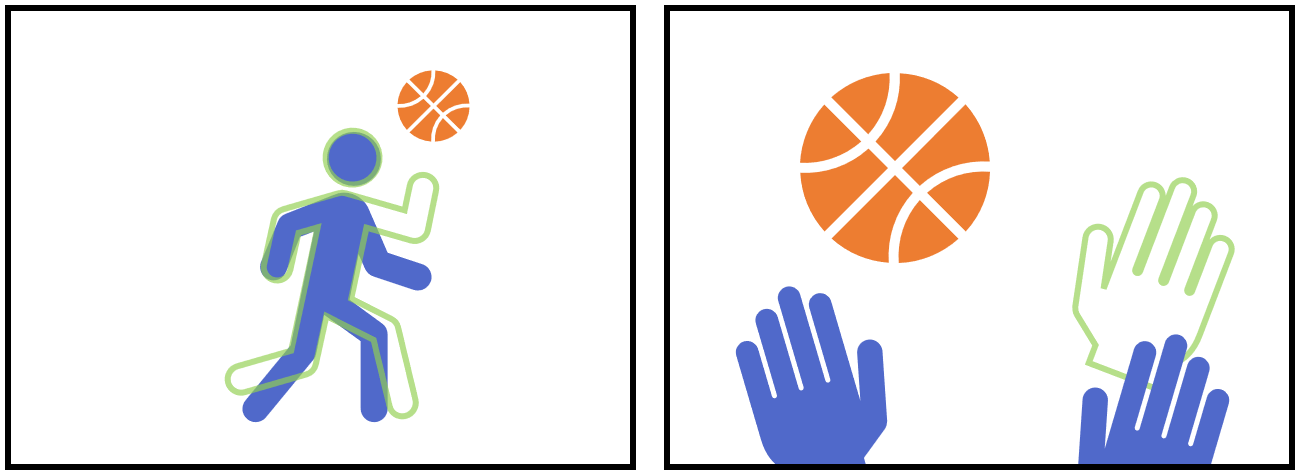
\includegraphics[width=\linewidth]{pictures/PointOfView.PNG}
    \caption[Comparison of an exocentric and egocentric perspective.]{A person exercising with a ball. Exocentric (left) and egocentric (right) view types with possible target movement (feedback) in red and the actual movement in black.\label{fig:POV}}
\end{figure}


\subsection*{Abstraction Type}
The \textit{abstraction type} of movement information used for giving feedback impacts the users' experience and the corrections they execute. \textit{Directional feedback} shows the direction in which a limb should be corrected. For example, arrows can be utilized to achieve this. An alternative to showing the correcting movement is to visualize the target state. \textit{Positional feedback} predominantly does this with an outline, transparent target avatar, or end position to show where the ideal position is. In contrast to that, \textit{guidance} demonstrates the desired movement before the user will execute it. The concrete visual cues being used to provide these types of information are described in \autoref{sec:visualCues}.

\subsection*{Temporal Order}
The \textit{temporal order} in which the feedback is provided in the context of the movement execution varies in the analyzed approaches. In some cases, a \textit{playback}, where the feedback is shown after the execution, might increase the precision of movement, while in other cases a \textit{real time} feedback offers an instantaneous in-situ opportunity to apply correction. Additionally, it is possible to show the user the future movements, which can provide information about \textit{upcoming} target motions.

\subsection*{Stages of Learning}
Considering that motor feedback can help users learn a skill, Fitts and Posner's \cite{fitts1967HPe} stages of learning can be applied to visual motor feedback.
We use the feedback features provided by the surveyed literature to assign each approach to one of the \textit{stages of learning}. This assignment can provide useful information regarding which part of the learning process the feedback addresses and which depth it can provide. The stages are explained in more detail in \autoref{sec:stages}. It is also to be said, that the stages are transitioning into each other fluently and that in some cases arguments for a classification into a different category can be made \cite{fitts1967HPe}. 

\subsection*{Publication Venue}
The literature surveyed is sourced from several different \emph{publication venues}. We categorized the venues as \emph{computer science (\acrshort{vr}, \acrshort{ar}, \acrshort{vr})}, \textit{computer science (HCI)}, \emph{computer science (other)}, \emph{medicine, health \& sports} as well as \emph{patents}. These categories can give readers a general orientation in which areas most of the research is rooted and where there is still potential. The descriptions from authors from different venues also usually put emphasis on different parts of the respective approaches (e.\,g. application vs. technology vs. usefulness).

\subsection*{Body Parts}
Furthermore, the \textit{body parts} for which feedback is given are of interest. The feedback changes with the degrees of freedom of different joints. It is also interesting to consider how the visibility of a body part in a neutral position interacts with the feedback (see \autoref{sec:POV}). In the literature we surveyed, the feedback was provided for \textit{arms}, \textit{legs}, \textit{hands}, or the \textit{whole body}.

\begin{figure*}[tb]
    \centering
    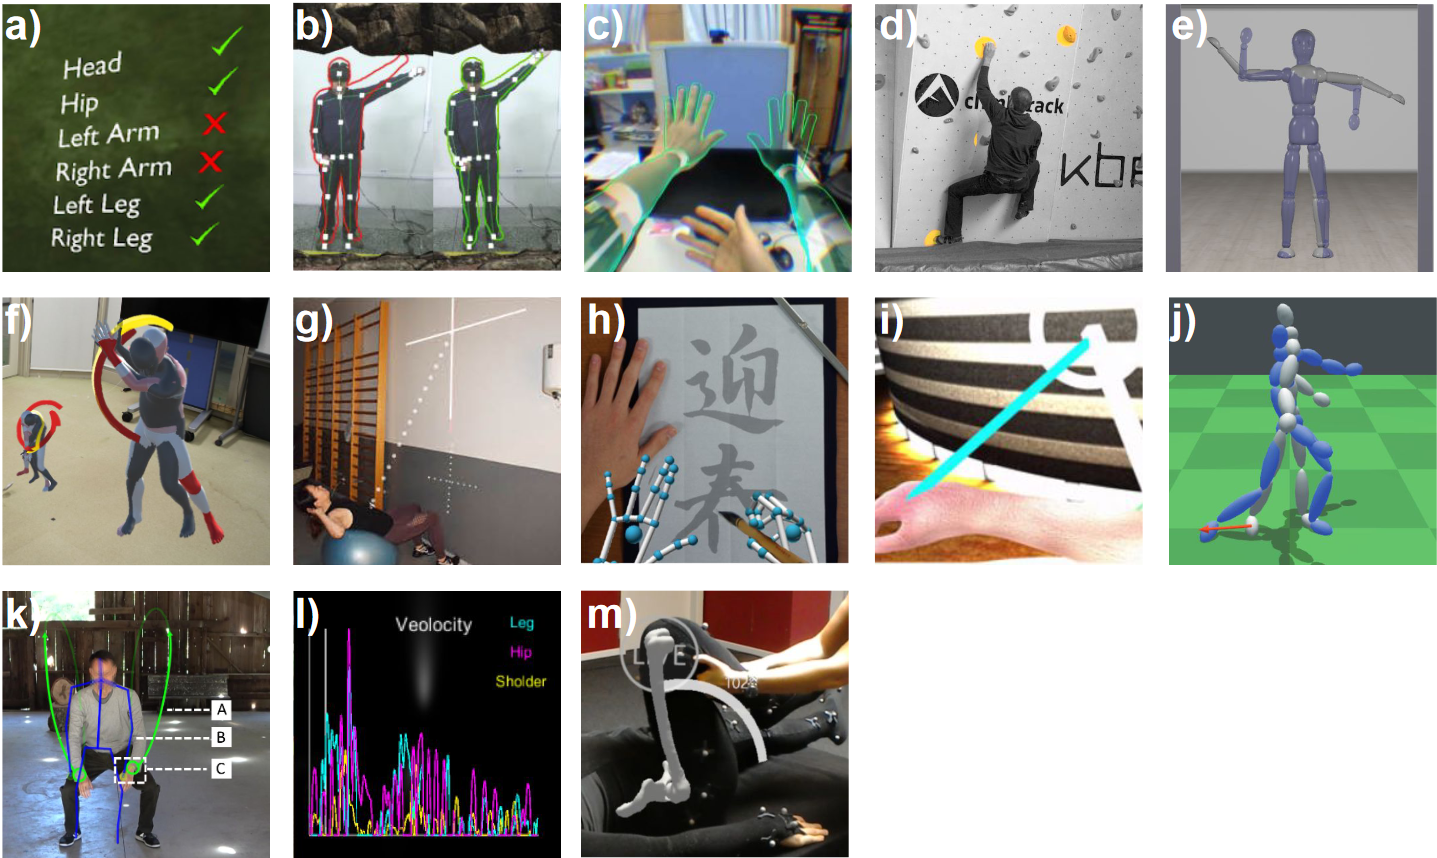
\includegraphics[width=1\linewidth]{pictures/CueMatrix.PNG}
    \caption[Examples of visual cues used in the literature.]{Examples of visual cues used in the literature and described in~\autoref{sec:visualCues}: a) Textual, b) Color coding, c) Body outline, d) End position, e) Transparent target avatar, f) Opaque target avatar, g) Abstraction, h) Video overlay, i) Rubber bands, j) Arrows, k) Trajectories, l) Graphs, m) Limb angles.  Images from \cite{caserman2021fbm}, \cite{quevedo2017asr}, \cite{han2016ara}, \cite{wiehr2016bce}, \cite{waltemate2016tlp}, \cite{ikeda2018arb}, \cite{vidal2020blo}, \cite{furukawa2018dar}, \cite{yu2020pmd}, \cite{oshita2018sts}, \cite{clarke2020rva}, \cite{takahashi2019vrb}, \cite{debarba2018arv}. \label{fig:CueMatrix}}
\end{figure*}

\subsection*{Use Case}
The analyzed approaches showed a wide variety of use cases the feedback was given for. We identified \textit{individual sports}, \textit{team sports}, \textit{rehabilitation}, and \textit{motor skill training} as typical use cases. \textit{Motor skill training}, here, does not only include approaches that analyzed motor skill training \emph{per se}, but also the ones that had no use case taken into consideration so far.


\subsection*{Visual Cues \label{sec:visualCues}}
The visualizations in the literature surveyed featured several different \textit{visual cues} to indicate how a target movement should be executed. These visual cues are the most in-depth description of the feedback we provide and are closely linked to other features such as technology, body parts, and use cases. The distribution of visual cues among the literature surveyed is listed in \autoref{table:2}. Exemplary images for all the visual cues explained in the following can be found in \autoref{fig:CueMatrix}. The labels of the examples in  \autoref{fig:CueMatrix} correspond to the letters found in front of the visual cue names in the following description.

\begin{table*}[thp]\centering
    \begin{tiny}
    \caption[Classification of reviewed literature.]{Classification of reviewed literature. Explanation for classification features can be found in \autoref{sec:classification}. Visual cues are explained in \autoref{sec:visualCues}.\label{table:2}}
    \setlength\tabcolsep{2.1pt}
    \setlength\extrarowheight{5pt}
    \resizebox{\linewidth}{!}{
\begin{tabular}{|c|r|c|c|c|c|c|c|c|c|c|c|c|c|c|c|c|c|c|c|c|c|c|c|c|c|c|c|c|c|c|c|c|c|c|c|c|c|c|c|c|c|}
\hline
& Authors & \rotatebox[origin=l]{90}{Oka et al.} & \rotatebox[origin=l]{90}{Ikeda et al.} & \rotatebox[origin=l]{90}{Wiehr et al.} & \rotatebox[origin=l]{90}{Afyouni et al.} & \rotatebox[origin=l]{90}{Cao et al.} & \rotatebox[origin=l]{90}{Ikeda et al.} & \rotatebox[origin=l]{90}{Han et al.} & \rotatebox[origin=l]{90}{Quevedo et al.} & \rotatebox[origin=l]{90}{Debarba et al.} & \rotatebox[origin=l]{90}{Barioni et al.} & \rotatebox[origin=l]{90}{Vidal et al.} & \rotatebox[origin=l]{90}{Kosmalla et al.} & \rotatebox[origin=l]{90}{Raffe et al.} & \rotatebox[origin=l]{90}{Conner and Poor} & \rotatebox[origin=l]{90}{Furukawa et al.} & \rotatebox[origin=l]{90}{Marti} & \rotatebox[origin=l]{90}{Escalona et al.} & \rotatebox[origin=l]{90}{Caserman et al.} & \rotatebox[origin=l]{90}{Booth et al.} & \rotatebox[origin=l]{90}{Shiro et al.} & \rotatebox[origin=l]{90}{Pereira et al.} & \rotatebox[origin=l]{90}{Meyer et al.} & \rotatebox[origin=l]{90}{Han et al.} & \rotatebox[origin=l]{90}{Hoang et al.} & \rotatebox[origin=l]{90}{Yu et al.} & \rotatebox[origin=l]{90}{Sekhavat et al.} & \rotatebox[origin=l]{90}{Clarke et al.} & \rotatebox[origin=l]{90}{Oshita et al.} & \rotatebox[origin=l]{90}{Murlowski et al.} & \rotatebox[origin=l]{90}{Sousa et al.} & \rotatebox[origin=l]{90}{Hülsmann et al.} & \rotatebox[origin=l]{90}{Naour et al.} & \rotatebox[origin=l]{90}{Trajkova et al.} & \rotatebox[origin=l]{90}{Waltemate et al.} & \rotatebox[origin=l]{90}{Booth et al.} & \rotatebox[origin=l]{90}{Karatsidis et al.} & \rotatebox[origin=l]{90}{Takahashi et al.} & \rotatebox[origin=l]{90}{Mostajeran et al.} & \rotatebox[origin=l]{90}{Ware et al.} & \rotatebox[origin=l]{90}{Row count in \%} \\
\hline
 & Reference & \rotatebox[origin=c]{90}{\cite{oka2021rtf}} & \rotatebox[origin=c]{90}{\cite{ikeda2019rtp}} & \rotatebox[origin=c]{90}{\cite{wiehr2016bce}} & \rotatebox[origin=c]{90}{\cite{afyouni2020arb}} & \rotatebox[origin=c]{90}{\cite{cao2020esa}} & \rotatebox[origin=c]{90}{\cite{ikeda2018arb}} & \rotatebox[origin=c]{90}{\cite{han2016ara}} & \rotatebox[origin=c]{90}{\cite{quevedo2017asr}} & \rotatebox[origin=c]{90}{\cite{debarba2018arv}} & \rotatebox[origin=c]{90}{\cite{barioni2019bvr}} & \rotatebox[origin=c]{90}{\cite{vidal2020blo}} & \rotatebox[origin=c]{90}{\cite{kosmalla2017cvi}} & \rotatebox[origin=c]{90}{\cite{raffe2018cst}} & \rotatebox[origin=c]{90}{\cite{conner2016cef}} & \rotatebox[origin=c]{90}{\cite{furukawa2018dar}} & \rotatebox[origin=c]{90}{\cite{marti2019evl}} & \rotatebox[origin=c]{90}{\cite{escalona2020eva}} & \rotatebox[origin=c]{90}{\cite{caserman2021fbm}} & \rotatebox[origin=c]{90}{\cite{booth2019msr}} & \rotatebox[origin=c]{90}{\cite{shiro2019ipv}} & \rotatebox[origin=c]{90}{\cite{pereira2017jat}} & \rotatebox[origin=c]{90}{\cite{meyer2018jlc}} & \rotatebox[origin=c]{90}{\cite{han2017mtc}} & \rotatebox[origin=c]{90}{\cite{hoang2016orp}} & \rotatebox[origin=c]{90}{\cite{yu2020pmd}} & \rotatebox[origin=c]{90}{\cite{sekhavat2018pba}} & \rotatebox[origin=c]{90}{\cite{clarke2020rva}} & \rotatebox[origin=c]{90}{\cite{oshita2018sts}} & \rotatebox[origin=c]{90}{\cite{brewster2019srt}} & \rotatebox[origin=c]{90}{\cite{sousa2016sar}} & \rotatebox[origin=c]{90}{\cite{huelsmann2019ssp}} & \rotatebox[origin=c]{90}{\cite{naour2019s3d}} & \rotatebox[origin=c]{90}{\cite{trajkova2018ttb}} & \rotatebox[origin=c]{90}{\cite{waltemate2016tlp}} & \rotatebox[origin=c]{90}{\cite{booth2019vue}} & \rotatebox[origin=c]{90}{\cite{karatsidis2018vwv}} & \rotatebox[origin=c]{90}{\cite{takahashi2019vrb}} & \rotatebox[origin=c]{90}{\cite{mostajeran2019hvc}} & \rotatebox[origin=c]{90}{\cite{ware2020wo2}} & \\ \hline \hline
\multirow{6}{*}{\rotatebox[origin=c]{90}{\acrshort{vr} technologies}} & Optical see-through &  &  &  &  &  & $\bullet$ &  &  & $\bullet$ &  &  & $\bullet$ &  &  &  &  &  &  &  &  &  & $\bullet$ & $\bullet$ &  &  &  &  &  &  &  &  &  &  &  &  & $\bullet$ &  &  &  & 15.4 \\ \cline{2-42}
 & Video see-through &  &  &  &  & $\bullet$ &  & $\bullet$ &  &  &  &  &  &  &  &  &  &  &  &  &  &  &  &  &  &  &  &  &  &  &  &  &  &  &  &  &  &  & $\bullet$ &  & 7.7 \\ \cline{2-42}
 & Projection &  & $\bullet$ & $\bullet$ &  &  &  &  &  &  &  & $\bullet$ & $\bullet$ &  &  &  &  &  &  &  &  &  &  &  &  &  & $\bullet$ &  &  &  & $\bullet$ &  &  &  &  &  &  &  &  &  & 15.4 \\ \cline{2-42}
 & \acrshort{cave} &  &  &  &  &  &  &  &  &  &  &  &  &  &  &  &  &  &  &  &  &  &  &  &  &  &  &  &  &  &  & $\bullet$ &  &  &  &  &  &  &  &  & 2.6 \\ \cline{2-42}
 & \acrshort{vr} glasses & $\bullet$ &  &  & $\bullet$ &  & $\bullet$ &  & $\bullet$ &  &  &  &  & $\bullet$ &  & $\bullet$ &  &  & $\bullet$ &  &  &  &  &  & $\bullet$ & $\bullet$ &  &  &  &  &  &  &  &  &  &  &  & $\bullet$ &  & $\bullet$ & 28.2 \\ \cline{2-42}
 & \acrshort{rmd} &  &  &  &  &  &  &  &  &  & $\bullet$ &  &  &  & $\bullet$ &  & $\bullet$ & $\bullet$ &  & $\bullet$ & $\bullet$ & $\bullet$ &  &  &  &  &  & $\bullet$ & $\bullet$ & $\bullet$ &  &  & $\bullet$ & $\bullet$ & $\bullet$ & $\bullet$ &  &  &  &  & 35.9 \\ \hline \hline
\multirow{4}{*}{\rotatebox[origin=c]{90}{\Acrshort{pov}}} & First person &  &  & $\bullet$ &  & $\bullet$ &  & $\bullet$ &  & $\bullet$ &  & $\bullet$ & $\bullet$ &  &  & $\bullet$ &  &  &  &  &  &  & $\bullet$ & $\bullet$ & $\bullet$ &  & $\bullet$ &  &  &  & $\bullet$ &  &  &  &  &  & $\bullet$ & $\bullet$ &  & $\bullet$ & 38.5 \\ \cline{2-42} 
 & Third person & $\bullet$ & $\bullet$ &  & $\bullet$ &  &  &  & $\bullet$ &  & $\bullet$ &  &  &  & $\bullet$ &  & $\bullet$ & $\bullet$ &  & $\bullet$ & $\bullet$ & $\bullet$ &  &  &  &  &  & $\bullet$ & $\bullet$ & $\bullet$ &  & $\bullet$ & $\bullet$ & $\bullet$ & $\bullet$ & $\bullet$ &  & $\bullet$ & $\bullet$ & & 53.8 \\ \cline{2-42} 
 & Both &  &  &  &  &  & $\bullet$ &  &  &  &  &  &  & $\bullet$ &  &  &  &  & $\bullet$ &  &  &  &  &  &  & $\bullet$ &  &  &  &  &  &  &  &  &  &  &  &  &  &  & 10.3 \\ \cline{2-42} 
 & For instructor &  &  &  &  &  &  &  &  & $\bullet$ &  &  &  &  &  & $\bullet$ &  &  &  &  &  &  &  &  &  &  &  &  &  &  &  &  &  &  &  &  &  &  &  &  & 5.1 \\ \hline \hline
\multirow{3}{*}{\rotatebox[origin=c]{90}{\parbox{1cm}{\centering Abstraction Type}}} & Directional &  &  &  &  &  &  &  &  &  &  &  &  &  &  &  &  &  &  &  & $\bullet$ &  & $\bullet$ &  &  & $\bullet$ &  &  & $\bullet$ &  &  &  &  &  &  &  &  &  &  &  & 10.3 \\ \cline{2-42}
 & Positional & $\bullet$ & $\bullet$ & $\bullet$ & $\bullet$ &  & $\bullet$ &  & $\bullet$ & $\bullet$ & $\bullet$ & $\bullet$ & $\bullet$ & $\bullet$ & $\bullet$ &  & $\bullet$ & $\bullet$ & $\bullet$ & $\bullet$ & $\bullet$ & $\bullet$ &  &  & $\bullet$ & $\bullet$ & $\bullet$ & $\bullet$ & $\bullet$ &  & $\bullet$ & $\bullet$ & $\bullet$ & $\bullet$ & $\bullet$ & $\bullet$ & $\bullet$ & $\bullet$ &  &  & 76.9 \\ \cline{2-42} 
 & Guidance &  &  &  &  & $\bullet$ &  & $\bullet$ &  &  &  &  & $\bullet$ &  &  & $\bullet$ &  &  &  &  &  &  &  & $\bullet$ &  &  &  &  &  & $\bullet$ &  &  &  &  &  &  &  &  & $\bullet$ & $\bullet$ & 20.5 \\ \hline \hline
\multirow{3}{*}{\rotatebox[origin=c]{90}{\parbox{1cm}{\centering Temporal order}}} & Playback &  &  &  &  &  & $\bullet$ &  &  &  &  &  &  &  & $\bullet$ &  &  & $\bullet$ &  &  & $\bullet$ & $\bullet$ & $\bullet$ &  &  &  &  &  & $\bullet$ &  &  &  & $\bullet$ &  &  &  &  & $\bullet$ &  &  & 23.1 \\ \cline{2-42} 
 & Real time & $\bullet$ & $\bullet$ &  & $\bullet$ &  & $\bullet$ &  & $\bullet$ & $\bullet$ & $\bullet$ & $\bullet$ &  &  &  & $\bullet$ & $\bullet$ &  & $\bullet$ & $\bullet$ &  &  &  & $\bullet$ & $\bullet$ &  &  & $\bullet$ &  &  & $\bullet$ & $\bullet$ &  & $\bullet$ & $\bullet$ & $\bullet$ & $\bullet$ &  &  & $\bullet$ & 56.4 \\ \cline{2-42} 
 & Upcoming &  &  & $\bullet$ &  & $\bullet$ &  & $\bullet$ &  &  &  &  & $\bullet$ & $\bullet$ &  &  &  & $\bullet$ &  &  &  &  &  &  &  & $\bullet$ & $\bullet$ &  & $\bullet$ & $\bullet$ &  &  & $\bullet$ &  &  &  &  &  & $\bullet$ & $\bullet$ & 33.3 \\ \hline \hline
\multirow{3}{*}{\rotatebox[origin=c]{90}{\parbox{1.2 cm}{\centering Stages of learning}}} & Cognitive &  &  &  &  & $\bullet$ &  & $\bullet$ & $\bullet$ &  & $\bullet$ &  & $\bullet$ & $\bullet$ &  & $\bullet$ &  & $\bullet$ &  &  &  &  & $\bullet$ & $\bullet$ & $\bullet$ & $\bullet$ & $\bullet$ & $\bullet$ & $\bullet$ & $\bullet$ & $\bullet$ &  &  &  & $\bullet$ & $\bullet$ &  &  & $\bullet$ & $\bullet$ & 53.8 \\ \cline{2-42}
 & Associative & $\bullet$ & $\bullet$ & $\bullet$ & $\bullet$ & $\bullet$ & $\bullet$ &  &  & $\bullet$ & $\bullet$ & $\bullet$ & $\bullet$ &  & $\bullet$ & $\bullet$ &  & $\bullet$ & $\bullet$ & $\bullet$ & $\bullet$ & $\bullet$ & $\bullet$ & $\bullet$ & $\bullet$ & $\bullet$ &  & $\bullet$ & $\bullet$ &  &  & $\bullet$ & $\bullet$ & $\bullet$ & $\bullet$ & $\bullet$ & $\bullet$ &  & $\bullet$ & $\bullet$ & 82.1 \\ \cline{2-42} 
 & Autonomous &  &  &  & $\bullet$ &  & $\bullet$ &  &  & $\bullet$ &  &  &  &  &  &  & $\bullet$ &  &  &  &  & $\bullet$ &  &  &  &  &  &  &  &  &  &  &  &  &  &  & $\bullet$ & $\bullet$ &  &  & 17.9 \\ \hline \hline
\multirow{5}{*}{\rotatebox[origin=c]{90}{\parbox{1cm}{\centering Publication venue}}} & Comp. sc. (\acrshort{vr}, \acrshort{ar}, \acrshort{vr}) &  & $\bullet$ &  &  &  & $\bullet$ & $\bullet$ & $\bullet$ & $\bullet$ & $\bullet$ &  &  &  &  &  &  & $\bullet$ & &  & $\bullet$  &  &  & $\bullet$ &  & $\bullet$ &  &  & $\bullet$ &  &  & &  &  & $\bullet$ &  &  & $\bullet$ & $\bullet$ &  & 35.9 \\ \cline{2-42} 
 & Comp. sc. (HCI) &  &  & $\bullet$ &  & $\bullet$ &  &  &  &  &  & $\bullet$  & $\bullet$  &  & $\bullet$ &  &  &  &  &  &  &  & $\bullet$ &  & $\bullet$ &  & $\bullet$ & $\bullet$ &  & $\bullet$ & $\bullet$ &  &  &  &  &  & &  &  &  & 28.2 \\ \cline{2-42} 
 & Comp. sc. (others) & $\bullet$ &  &   &$\bullet$  &  &  &  &  &  &  &  &  &  &  & $\bullet$ &  &  & $\bullet$   &  &  &  &  &  &  &  &  &  &  &  &  & $\bullet$ & $\bullet$ & $\bullet$ &  &  & &  &  &  & 17.9 \\ \cline{2-42} 
 & Medicine, health \& sports&  &  &  &  &  &  &  &  &  &  &  &  & $\bullet$ &  &  & $\bullet$ &  &  & $\bullet$ &  & $\bullet$ &  &  &  &  &  &  &  &  &  &  &  &  &  & $\bullet$ & $\bullet$ &  &  &  & 15.4 \\ \cline{2-42} 
 & Patent &  &  &  &  &  &  &  &  &  &  &  &  &  &  &  &  &  &  &  &  &  &  &  &  &  &  &  &  &  &  &  &  &  &  &  &  &  &  & $\bullet$ & 2.6 \\ \hline \hline
\multirow{4}{*}{\rotatebox[origin=c]{90}{Body parts}} & Whole body & $\bullet$ & $\bullet$ &  & $\bullet$ & $\bullet$ & $\bullet$ &  & $\bullet$ &  & $\bullet$ & $\bullet$ & $\bullet$ &  & $\bullet$ &  &  & $\bullet$ & $\bullet$ &  & $\bullet$ & $\bullet$ &  & $\bullet$ & $\bullet$ &  &  & $\bullet$ & $\bullet$ & $\bullet$ &  & $\bullet$ & $\bullet$ & $\bullet$ & $\bullet$ & $\bullet$ &  & $\bullet$ & $\bullet$ & $\bullet$ & 69.2 \\ \cline{2-42} 
 & Arms &  &  & $\bullet$ &  &  &  & $\bullet$ &  &  &  &  &  &  &  &  &  &  &  &  &  &  & $\bullet$ &  &  & $\bullet$ &  &  &  &  & $\bullet$ &  &  &  &  &  &  &  &  &  & 12.8 \\ \cline{2-42} 
 & Legs &  &  & $\bullet$ &  &  &  &  &  & $\bullet$ &  &  &  & $\bullet$ &  &  & $\bullet$ &  &  & $\bullet$ &  &  &  &  &  &  & $\bullet$ &  &  &  &  &  &  &  &  &  & $\bullet$ &  &  &  & 17.9 \\ \cline{2-42} 
 & Hands &  &  &  &  &  &  &  &  &  &  &  &  &  &  & $\bullet$ &  &  &  &  &  &  &  &  &  &  &  &  &  &  &  &  &  &  &  &  &  &  &  &  & 2.6 \\ \hline \hline
\multirow{4}{*}{\rotatebox[origin=c]{90}{Use case}} & Individual sports & $\bullet$ & $\bullet$ & $\bullet$ &  &  & $\bullet$ & $\bullet$ &  &  & $\bullet$ & $\bullet$ & $\bullet$ &  &  &  & $\bullet$ &  & $\bullet$ &  & $\bullet$ &  & $\bullet$ & $\bullet$ &  &  &  &  & $\bullet$ & $\bullet$ &  &  &  & $\bullet$ &  &  &  &  &  & $\bullet$ & 43.6 \\ \cline{2-42} 
 & Team sports &  &  &  &  &  &  &  &  &  &  &  &  &  &  &  &  &  &  &  &  &  &  &  &  &  &  &  &  &  &  &  & $\bullet$ &  &  &  &  & $\bullet$ &  &  & 5.1 \\ \cline{2-42} 
 & Rehabilitation &  &  &  & $\bullet$ &  &  &  & $\bullet$ & $\bullet$ &  &  &  & $\bullet$ &  &  &  & $\bullet$ &  & $\bullet$ &  & $\bullet$ &  &  &  &  & $\bullet$ &  &  &  & $\bullet$ &  &  &  &  & $\bullet$ & $\bullet$ &  & $\bullet$ &  & 30.8 \\ \cline{2-42} 
 & Motor skill training &  &  &  &  & $\bullet$ &  &  &  &  &  &  &  &  & $\bullet$ & $\bullet$ &  &  &  &  &  &  &  &  & $\bullet$ & $\bullet$ &  & $\bullet$ &  &  &  & $\bullet$ &  &  & $\bullet$ &  &  &  &  &  & 20.5 \\ \hline \hline
\multirow{13}{*}{\rotatebox[origin=c]{90}{Visual Cues}}
 & Textual & $\bullet$ &  &  & $\bullet$ &  &  &  &  &  &  &  &  &  & $\bullet$ &  &  &  & $\bullet$ &  &  &  &  &  &  &  &  &  & $\bullet$ & $\bullet$ &  &  &  & $\bullet$ &  &  &  &  &  &  & 17.9 \\ \cline{2-42} 
 & Color Coding & $\bullet$ &  &  &  &  &  &  & $\bullet$ &  &  &  &  &  & $\bullet$ &  &  &  &  & $\bullet$ &  &  &  &  &  &  & $\bullet$ &  &  &  &  &  &  &  & $\bullet$ &  & $\bullet$ &  &  &  & 17.9 \\ \cline{2-42} 
 & Body Outline &  & $\bullet$ &  &  &  &  & $\bullet$ & $\bullet$ &  &  &  &  &  &  &  &  &  &  &  &  &  &  &  &  &  &  &  &  &  &  &  &  &  &  &  &  &  &  &  & 7.7 \\ \cline{2-42} 
 & End Position &  &  & $\bullet$ &  &  &  &  &  &  &  &  & $\bullet$ & $\bullet$ &  &  &  &  &  & $\bullet$ &  &  &  &  &  & $\bullet$ & $\bullet$ &  &  &  &  &  &  & $\bullet$ &  & $\bullet$ &  &  &  &  & 20.5 \\ \cline{2-42} 
 & Transparent Target Avatar &  &  &  & $\bullet$ & $\bullet$ &  &  &  &  & $\bullet$ &  &  &  &  &  &  &  &  &  &  &  &  &  & $\bullet$ &  &  &  &  &  &  & $\bullet$ &  &  & $\bullet$ &  &  &  &  &  & 15.4 \\ \cline{2-42} 
 & Opaque Target Avatar &  &  &  &  &  & $\bullet$ &  &  &  &  &  & $\bullet$ &  &  &  &  & $\bullet$ &  &  &  &  &  & $\bullet$ & $\bullet$ &  &  &  & $\bullet$ &  &  &  & $\bullet$ &  &  &  &  &  & $\bullet$ &  & 20.5 \\ \cline{2-42} 
 & Movement Abstraction &  &  &  &  &  &  &  &  &  &  & $\bullet$ &  &  &  &  & $\bullet$ &  &  & $\bullet$ &  &  & $\bullet$ &  &  &  &  &  &  &  & $\bullet$ &  &  &  &  &  & $\bullet$ &  &  &  & 15.4 \\ \cline{2-42} 
 & Video Overlay &  &  &  &  &  &  &  & $\bullet$ &  &  &  & $\bullet$ &  &  & $\bullet$ &  & $\bullet$ &  &  & $\bullet$ &  &  &  &  &  &  & $\bullet$ &  &  &  &  &  &  &  &  &  &  &  & $\bullet$ & 17.9 \\ \cline{2-42} 
 & Rubber Bands &  &  &  &  &  &  &  &  &  &  &  &  &  &  &  &  &  &  &  &  &  &  &  &  & $\bullet$ &  &  &  &  &  &  &  &  &  &  &  &  &  &  & 2.6 \\ \cline{2-42} 
 & Arrows &  &  &  &  &  &  &  &  &  &  &  &  &  &  &  &  &  &  &  &  &  &  &  &  & $\bullet$ &  &  & $\bullet$ &  &  &  &  &  &  &  &  &  &  &  & 5.1 \\ \cline{2-42} 
 & Trajectories &  &  &  &  &  & $\bullet$ &  &  &  &  &  &  &  &  &  &  &  &  &  &  & $\bullet$ &  &  &  &  &  & $\bullet$ &  &  &  &  &  &  &  &  &  &  &  &  & 7.7 \\ \cline{2-42} 
& Graphs &  &  &  &  &  &  &  &  &  &  &  &  &  &  &  &  &  &  &  &  & $\bullet$ &  &  &  &  &  &  &  &  &  &  &  &  &  &  &  & $\bullet$ &  &  & 5.1 \\ \cline{2-42} 
& Limb Angles &  &  &  &  &  &  &  &  & $\bullet$ &  &  &  &  &  &  &  &  &  &  &  &  &  &  &  &  &  &  & $\bullet$ &  &  &  &  &  &  &  &  &  &  &  & 5.1 \\ \cline{2-42}
\hline
\end{tabular}
}
\end{tiny}
\end{table*}

\textbf{a) Textual}

Hints to correct the movement with words or text were categorized as \textit{textual}. These cues are in most cases combined with other feedback methods (\eg\ Oshita et al. \cite{oshita2018sts} and Conner and Poor \cite{conner2016cef}).

\textbf{b) Color Coding}

Colors can be an intuitive indicator of wrong or right (\eg\ red/green). For example an avatar with color-changing limbs or joints (as in \autoref{fig:Oka} taken from the work of Oka et al.~\cite{oka2021rtf}) can be used to give feedback for a desired movement. The \textit{color coding} can be utilized in many ways but is especially well suited to be used with a 2D or 3D avatar.

\textbf{c) Body Outline}

An outline of the body, or certain parts of it, can provide feedback while causing limited or no occlusion of an avatar or video that represents the actual position. Showing a \textit{body outline} is used in combination with video or avatars in both 3D and 2D. Ikeda et al.~\cite{ikeda2019rtp}, for instance, utilize this technique to give feedback for golf strikes.

\textbf{d) End Position}

To show the direction or correction of a movement it is possible to show the \textit{end positions} of certain limbs or joints. This advises the users to correct their pose so their limbs or joints fit these particular positions. Each end position is represented by a spatial coordinate. Oftentimes a volume or area is shown to allow for a certain tolerance. There are several methods implementing this, including 3D and 2D and even projection-based approaches (\eg\ Sekhavat et al.~\cite{sekhavat2018pba}).

\textbf{e) Transparent Target Avatar}

A \textit{transparent target avatar} can be used in combination with a video or 3D/2D opaque avatar showing the current pose to create a sense for how movements should be executed. The transparency of the target pose or target movement prevents this visual feedback from occluding the actual pose. For example, Barioni et al. demonstrate how this can be used to show target movements for ballet practice~\cite{barioni2019bvr}. This can be seen in \autoref{fig:Barioni}.

\textbf{f) Opaque Target Avatar}

In 3D, an \emph{opaque target avatar} depicting the target movement, can be superimposed with an avatar, showing the actual movement. The two objects colliding create an intersection effect as seen, \eg, in the work of Ikeda et al.~\cite{ikeda2018arb}. Another use of an opaque target avatar is a video overlay as seen for example in~\cite{kosmalla2017cvi}.

\textbf{g) Movement Abstraction}

The correction cues for some movements may be hard to perceive. This can be the case if the body part to be corrected is out of sight for the user or the correction and movement is minimal. These movements might be easier to comprehend if they are represented by an \textit{abstraction} of the movement rather than showing the actual movement or start/end position. An example of this is shown by Vidal et al.~\cite{vidal2020blo} in their work.

\textbf{h) Video Overlay}

If a video stream is implemented in the system it can be used to show a superimposed target avatar. This way the system can depict what movements to execute next, a sequence of movements, or correction cues. \textit{Video overlay} is used in \acrshort{ar} approaches and benefits from 3D implementation but is not limited to it. One example of this visual cue can be found in the work by Furukawa et al.~\cite{furukawa2018dar} who use video overlay to teach writing motions.

\textbf{i) Rubber Bands}

To indicate the direction of the target movement, the actual limb positions and the target limb position can be connected with a line. The result resembles so-called \textit{rubber bands} connecting actual and target body positions. Yu et al.~\cite{yu2020pmd} included this along with other visual cues in their approach.

\textbf{j) Arrows}

\textit{Arrows} are an intuitive technique to indicate a direction. Hence they can be used to show a direction in which to move or to provide correction cues for poses and movements. Oshita et al.~\cite{oshita2018sts}, for example, use it to show the direction in which the target pose lies.

It should be noted that arrows can be implemented as a special case of the above-mentioned rubber band cues. The only difference would be that an arrowhead is added.

\textbf{k) Trajectories}

Movements can be described by lines that represent the path of a certain joint or bone in space over time. These \textit{trajectories} can show the user where or along which path to move next, or how to correct the movement executed. Clarke et al.~\cite{clarke2020rva} combine trajectories with a video overlay in their approach.

\textbf{l) Graphs}

The data provided by the motion of a body can be used to create \textit{graphs} (sometimes also called \emph{plots}). This classical visualization of numerical data provides a detailed but abstract way to present movement information and correction cues to the user or instructor. As an example, Takahashi et al.~\cite{takahashi2019vrb} visualize the velocity of various joints and a ball to evaluate a baseball bat swing.

\textbf{m) Limb Angles}

One way of defining movements is by observing the angles at the joints between two bones. These \textit{limb angles} can consequently also be used to provide feedback to the user on how to correct the movement or in what way to move next (see \eg\ Debarba et al.~\cite{debarba2018arv}).





\section{Exemplary Discussion \label{sec:exemplary}}
In the following discussion, we will point out examples to explain certain features that are either widely spread among the surveyed literature or have rare occurrences. In other words, we provide a collection of \textit{representative} and \textit{exceptional} examples. This will help the reader understand the composition of the body of literature we are analyzing and will complement the overview provided by \autoref{table:2}.
\begin{figure}[h!t]
    \centering
    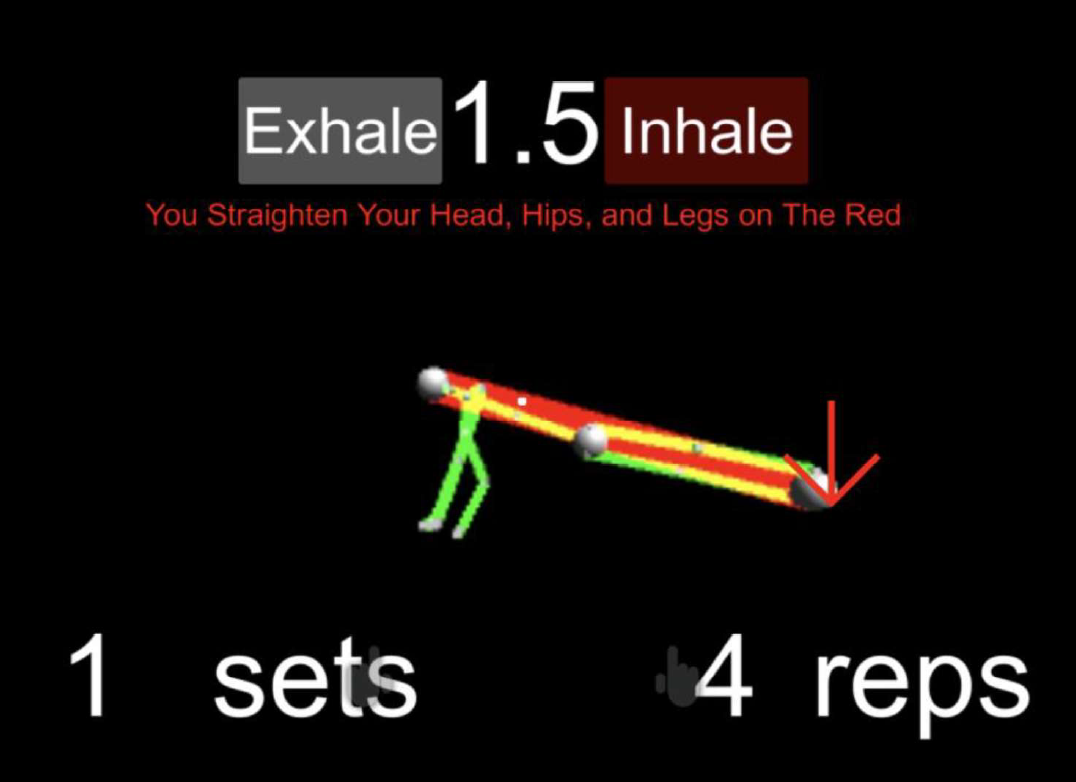
\includegraphics[width=0.6\linewidth]{pictures/Oka.PNG}
    \caption[Example of a color-coded skeleton.]{Color-coded skeleton: The skeleton visualizes where to correct the movement. Image from~\cite{oka2021rtf}.\label{fig:Oka}}
\end{figure}

\subsection{Representative Examples}
The work of Oka et al.~\cite{oka2021rtf} utilizes \emph{color coding} in their visualization to provide feedback to users through \emph{\acrshort{vr} glasses}. Users are shown color-coded cues indicating if any of their limbs need correction for an ideal execution of the exercise. The \emph{real time} feedback that is provided is supplemented by \emph{textual} cues and training metadata. The visualization of an abstracted skeleton as an avatar (see \autoref{fig:Oka}) is oftentimes utilized by the analyzed attempts (see for example Furukawa et al.~\cite{furukawa2018dar} or Escalona et al.~\cite{escalona2020eva}).


Ikeda et al.~\cite{ikeda2018arb} likewise present a research attempt to visualize motion feedback using \emph{\acrshort{vr} glasses}. Users can watch their body (as an avatar) from a \emph{third person} perspective. This enables them to gather information about the intended movement correction of the \emph{whole body}. It is possible to get the feedback in \emph{real time} as well as a \emph{playback} after the exercise. This work addresses the matching of actual and target movement with dynamic time warping. The matching of time discrepant executions is a challenge many real-time or playback feedback solutions have to face. The exocentric perspective in combination with \acrshort{vr} is a setup often found throughout the literature surveyed. An example can be found in the work of Hoang et al.~\cite{hoang2016orp} and Ware et al.~\cite{ware2020wo2}.

\begin{figure}[h!t]
    \centering
    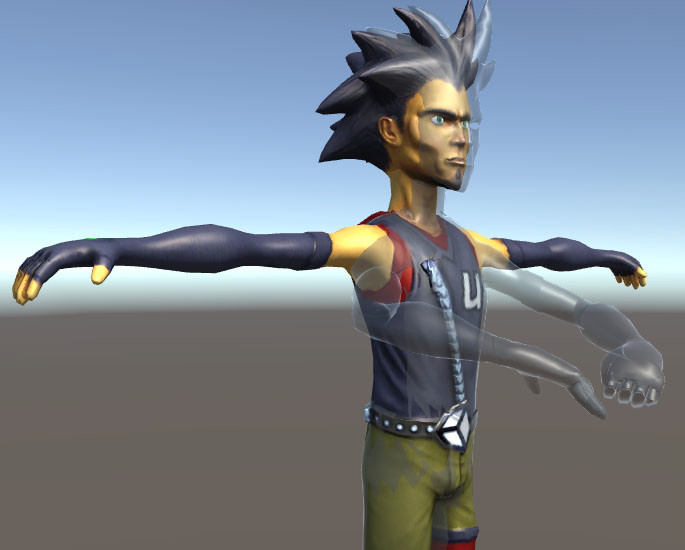
\includegraphics[width=0.6\linewidth]{pictures/Barioni.png}
    \caption[Transparent avatar for motion feedback.]{An opaque avatar shows the actual pose, while a transparent target avatar depicts the target pose, which is to be taken. Image from~\cite{barioni2019bvr}.\label{fig:Barioni}}
\end{figure}

Barioni et al.~\cite{barioni2019bvr} show \emph{upcoming} poses for the users to mimic. The target pose of the user is visualized by a \emph{transparent target avatar} which intersects an opaque avatar representing the user's actual pose (see \autoref{fig:Barioni}). The execution time of the pose is illustrated by a clock, which elapses when the pose is held correctly. The experimental setup uses an \acrshort{rmd} as feedback technology, but the system can also be used with \emph{\acrshort{vr} glasses}. The method of showing the poses before the execution is a typical way of providing information about the movement. It is often used in the literature at hand and can, for example, also be found in the work of Cao et al.~\cite{cao2020esa} and Han et al.~\cite{han2016ara}.


Oshita et al.~\cite{oshita2018sts} use \emph{opaque target avatars} to provide movement feedback for tennis shots. Additional \emph{arrows} show the \emph{direction} in which the correction is to be made and \emph{text} expresses how the movement should be executed. Furthermore, \emph{limb angles} are shown to depict the intended correction of a movement. After the execution, the feedback can be viewed on a large \emph{display}. The target avatar and avatars showing the actual user pose, together with the option of a \emph{playback} function is representative for many approaches in the surveyed literature. Examples of this combination can be found in the work of Hoang et al.~\cite{hoang2016orp} and Ikeda et al.~\cite{ikeda2018arb}. 

\subsection{Exceptional Examples}
A rehabilitation-oriented approach is presented by Debarba et al.~\cite{debarba2018arv}. With an \emph{optical see-through} \acrshort{hmd} they visualize realistic-looking bones of the clients. The \acrshort{hmd} is worn by the \emph{instructors}, who get \emph{real-time} feedback on how far the limb is bent by an angular indicator at the joint. The realistic rendering of bones is unique since it is often more legible to have abstract movement metaphors. Debarba et al. combine these realistic skeleton bones with a simple visualization of the \emph{limb angle}. This solution was chosen as an exceptional example due to the special circumstances of a rehabilitation setting in combination with the instructor as a feedback receiver.
\begin{figure}[h!t]
    \centering
    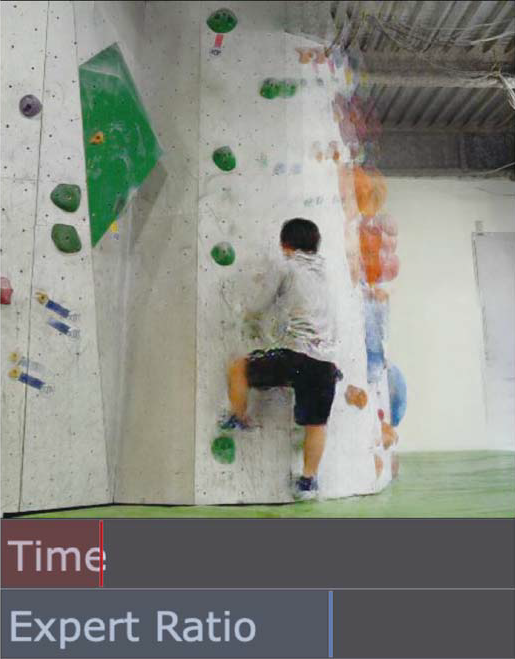
\includegraphics[height=0.4\linewidth]{pictures/Shiro.png}
    \caption[Synthesized frame between expert and beginner.]{Video frame synthesized by interpolating between user and expert pose. The upper slide bar represents the degree of expertise used for the interpolation. The lower slide bar controls the current frame of the playback. Image from~\cite{shiro2019ipv}.\label{fig:Shiro}}
\end{figure}

The work of Shiro et al.~\cite{shiro2019ipv} represents another innovative attempt at giving feedback for movements. The system generates a picture with an interpolation between the pose of the user and a recorded movement of an expert. After the movement execution, the user can set how close the generated image should resemble the expert movement and browse through the timeline of the \emph{playback} as seen in \autoref{fig:Shiro}. This interpolation and image synthesis technique is quite exceptional in the surveyed literature. It utilizes \acrfull{gan}, a \acrfull{ml} technique, to synthesize the images and show a \emph{target pose} for the user to imitate.


Vidal et al.~\cite{vidal2020blo} use a \emph{projection}-based approach to visualize the movement of the trunk. Lights attached to the body show the position of the trunk on the floor or walls of the room. The correct position is represented by a mark in the room. The users need to move to match this mark with the projected crosshair (see \autoref{fig:Vidal}). This \emph{abstract} approach, which works in \emph{real-time}, represents a singularity in the literature we analyzed.

Another approach utilizing \emph{projection} is presented by Kosmalla et al.~\cite{kosmalla2017cvi}. A projector displays an image on a climbing wall visualizing either the \emph{end position} of the next motion or an instructor performing the \emph{upcoming} movement. The attempt to project the feedback onto the training equipment is seen a few times throughout the literature. It is the scale and the virtual instructor on the wall that make this approach unique.
\begin{figure}[h!bt]
    \centering
    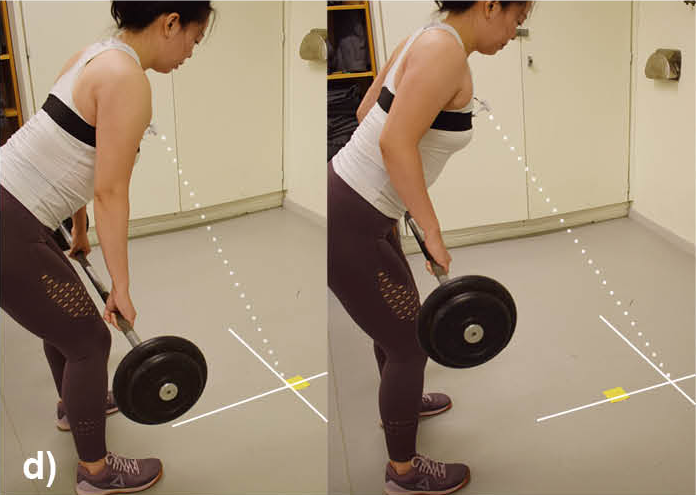
\includegraphics[width=0.6\linewidth]{pictures/Vidal.png}
    \caption[Projection-based \acrshort{vr} for body parts that are hard to see.]{Projection-based \acrshort{vr} for body parts that are hard to see. Assuming a correct movement execution the projected crosshair matches the marking on the floor. Image from~\cite{vidal2020blo}.\label{fig:Vidal}}
\end{figure}

\section{Survey Insights\label{sec:tvcg:insights}}
In this section, we will point out what we consider interesting findings of the classification seen in \autoref{table:2} and present what insights can be drawn from them. We discuss the insights by category.


\textbf{\emph{\acrshort{vr} Technologies:}} The most used \acrshort{vr} technology in the literature reviewed was \emph{\acrshort{rmd}s}, with \emph{\acrshort{vr}-glasses} in second place. The reason for \acrshort{rmd}s and \acrshort{vr} glasses as most used \acrshort{vr} technologies could be accredited to the fact that they are simple and inexpensive to implement. Especially \acrshort{rmd}s used as "augmented mirrors" (see \autoref{sec:MR}), as often seen in the literature surveyed, can be set up with little inexpensive equipment like a camera and a normal display. Additionally, an augmented mirror approach provides an intuitive way to receive full-body feedback.

Contrary to our expectations, optical see-through headsets made up a small percentage of 15.4\% of the used technologies. Despite the important development the HoloLens represents, not many approaches utilize it to give visual motor feedback to participants in physical therapy and exercise.

\textbf{\emph{\Acrshort{pov}:}} More than half of the approaches used a third-person view in their systems. This can be directly linked to the high quantity of \acrshort{rmd}s as all of these systems use a third-person perspective.

\textbf{\emph{Abstraction Type:}} A majority of research attempts we surveyed featured a positional form of feedback. It is noticeable that most directional feedback is a hybrid of directional and positional feedback. Pure directional feedback could be hard for humans to comprehend. Only showing the direction is insufficient information in many cases, as it would be difficult for the participant to stop at the target location. Information about the distance is crucial to be able to move correctly and precisely without further compensating motions.

\textbf{\emph{Stages of Learning:}} Regarding the learning phases, the literature was predominantly categorized into the \emph{associative} phase. Although the stages are overlapping and therefore a clear assignment is sometimes impossible, the dominance of the approaches that can be classified as \emph{associative} can still be seen as significant. It could be argued that visual feedback is most appropriate in the associative skill learning phase. When subroutines are put together to form one uniform skill or movement the motor feedback might be most effective and useful to the user.

When considering the connection between the visual cues and the learning stages, we came to the conclusion that using graphs as visual cues might be most suitable for learners already familiar with the skill. Such learners would be in the \emph{autonomous} stage. New learners might be overwhelmed with the detailed information, and it might not contribute to their improvement. Advanced users, already in the autonomous stage, might look for ways to improve their movement beyond their self-reliant execution and can therefore be supported with graphs. Additionally, a \emph{guidance} feedback type could be helpful for learners in the cognitive phase since the upcoming movement is demonstrated, and they can take in the information about the movement.

\textbf{\emph{Publication Venue:}} When looking at the publication venues, we can see that a majority (82.1\%) of papers were published in a computer science venue. As expected most of the publications were found in the \acrshort{vr}, \acrshort{ar}, and \acrshort{vr} sectors (35.9\%). Another substantial part (28.2\%) was found in the field of HCI. Furthermore, several (15.4\%) attempts were found in the fields of medicine, health, and sports. It is to mention here that research approaches in this sector often feature a different focus, for example, the medical state of the user or the impact of the system on performance. This sometimes culminates in the complete absence of statements or depictions regarding the visualizations employed in the publication. This led to an exclusion of such papers in the screening phase as described in \autoref{sec:tvcg:methodology}.

\textbf{\emph{Body Parts:}} Most feedback we observed was meant for the whole body. A few attempts concerned arms and legs and one paper covered feedback for hands. Again, it could be argued that this phenomenon is linked to the many examples of third-person augmented mirrors. Augmented mirrors are most suitable for a whole-body feedback type, as a mirror scenario is the most common way we experience the view of our whole body.

\textbf{\emph{Use Cases:}} The observation that many research attempts target individual sports seems trivial. \acrshort{hmd}s for example are limited to one user. To give clear feedback only one user can be addressed. If a whole team of participants would have to get feedback it would be either very time-consuming or many systems would have to be available simultaneously. However, in team sports the feedback for specific movements is traditionally given to the individual.

\textbf{\emph{Visual Cues:}} The most popular visual cues were \emph{end position} and \emph{opaque target avatar} as seen in \autoref{fig:CueHistogram}. The directional cues like \emph{arrows} and \emph{rubber bands} are seldom used throughout literature. The literature appears to prefer a positional approach.

\begin{figure}[h!tb]
    \centering
    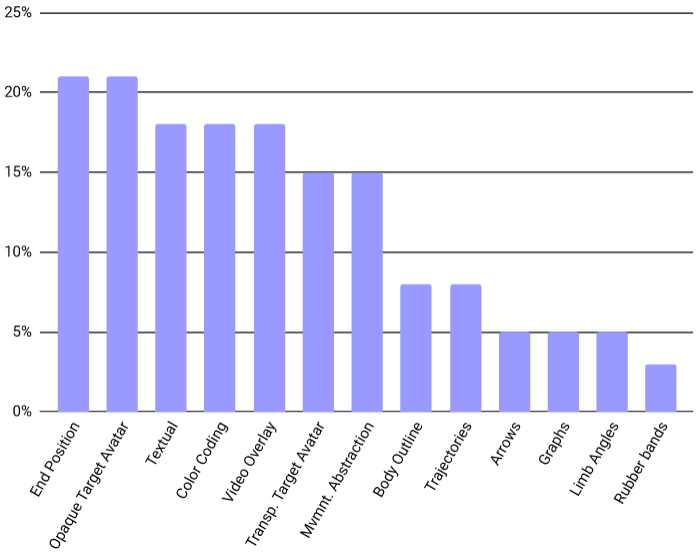
\includegraphics[width=0.8\linewidth]{pictures/CueHistogram.PNG}
    \caption{Occurrence of different visual cues in the selected literature.\label{fig:CueHistogram}}
\end{figure}

It becomes apparent that there are no clear outliers regarding the occurrences of visual cues. The literature does not seem to have found the best way to provide visual feedback in \acrshort{vr}. This can be attributed to the wide variety of different use cases appearing in the literature surveyed and to the diversity of movements associated to these use cases.

\textbf{\emph{Evaluation Methods:}} Various different approaches to evaluating the methods and technologies can be found in the literature surveyed. Evaluations were mostly conducted from a \emph{therapeutic}, \emph{user experience} or \emph{visualization} standpoint and usually included a user study. The \emph{therapeutic} evaluations were mainly concerned with the recovery of the user or patient. For example, Booth et al.\cite{booth2019msr} measured the step length, knee extension, and ankle power of participants. Aside from their work \cite{booth2019msr}\cite{booth2019vue}, Afyouni et al.~\cite{afyouni2020arb}, Marti~\cite{marti2019evl}, Sekhavat et al.~\cite{sekhavat2018pba} and Karatsidis et al.~\cite{karatsidis2018vwv} provide therapeutic evaluations of their work as well.

A \emph{user experience} focused evaluation was found in the work of Cao et al.~\cite{cao2020esa}, Barioni et al.~\cite{barioni2019bvr}, Han et al.~\cite{han2016ara}, Hoang et al.~\cite{hoang2016orp} and Mostajeran et al.~\cite{mostajeran2019hvc}. These evaluations usually include a questionnaire to identify the condition or opinion of the participants. For example, Barioni et al.~\cite{barioni2019bvr} developed a questionnaire involving ten questions regarding the use of their system to obtain an opinion from the participants.

Evaluations from the visualization standpoint often include measures like precision or correction times. We observed this for example in the work of Yu et al.~\cite{yu2020pmd}, who measured completion time and movement error. Aside from that, similar metrics can be found in the approaches of Cao et al.~\cite{cao2020esa}, Kosmalla et al.~\cite{kosmalla2017cvi}, Barioni et al.~\cite{hoang2016orp}, Sekhavat et al.~\cite{sekhavat2018pba}, Sousa et al.~\cite{sousa2016sar}, Hülsmann et al.~\cite{huelsmann2019ssp}, Naour et al.~\cite{naour2019s3d}, Tang et al.~\cite{tang2015pah}, Trajkova et al.~\cite{trajkova2018ttb} and Waltemate et al.~\cite{waltemate2016tlp}.

Not always a clear distinction of these perspectives is possible. There are some works analyzing the feedback system from several standpoints for example Cao et al.~\cite{cao2020esa} and Hoang et al.~\cite{hoang2016orp}. Several more evaluations were found among the surveyed literature, but they either had a very small number of participants (\cite{oshita2018sts}, \cite{meyer2018jlc}, \cite{escalona2020eva}, \cite{conner2016cef}) or did not deliver insights relevant for our overview (\cite{clarke2020rva}, \cite{han2016ara}, \cite{pereira2017jat}, \cite{caserman2021fbm}, \cite{vidal2020blo}, \cite{oka2021rtf}).

\section{Conclusion \label{sec:tvcg:conclusion}}
In this chapter, we gave an overview of the most recent literature on \acrshort{vr} feedback in the sector of physical exercise, rehabilitation, and general motor skill training. The literature has been classified and an overview of the classification is given in a table for easy reference. We discussed the different feedback types and identified potential for better utilization of feedback in the mentioned application areas.
We believe this survey closes a gap concerning a literature analysis by taking a closer look at visual cues. Furthermore, the survey could stimulate future research regarding visual cues for motor skill training as suggested in \autoref{sec:futureWork}.

\subsection{Findings}
We identified several trends:
\begin{itemize}
    \setlength{\itemsep}{-0.3cm}
    \item Many of the papers considered use approaches that can be described as virtual mirrors, that is a whole-body view on a display with feedback for certain movements.
    \item With respect to the abstraction type, positional feedback dominates the surveyed literature. Even directional feedback is often combined with the former to provide the user with sufficient information.
    \item In the examined approaches, feedback appeared to be mainly implemented for the associative skill learning phase.
    \item The papers used a variety of visual cues to pursue their goals. The most popular cues visualize the target pose or end position.
    \item The classification of literature in learning phases enables a more suitable feedback choice for specific target groups.
\end{itemize}

\subsection{Limitations}
This survey gives insight into which visual cues are utilized within the literature. We can only provide subtle hints to the reasons. An adequate analysis of the reasons for visual cue utilization is yet to be conducted. The chapter at hand does not deliver in-depth insights from a cognitive, therapeutic, or user experience standpoint.

As discussed in \autoref{sec:tvcg:methodology}, tool handling is not included in our scope. We solely focus on feedback for the human body. Nevertheless, several insights on visual cues and associated approaches might still be useful for supporting tool-based skill training with \acrshort{ar}.

There is no clear indication as to when Fitts and Posners~\cite{fitts1967HPe} learning phases apply, so the insights the classification can provide regarding this category are limited.

\subsection{Open Questions \label{sec:futureWork}}
At this state of research, the connection between feedback and learning stages~\cite{fitts1967HPe} is yet imprecise. It is still not always clear which visual cues are connected to which stages and what they invoke in users. It would be profitable to understand this connection better in order to improve motion learning in the sectors of rehabilitation, physical exercise, and private or professional skill training. With greater insight, the visual cues could be adjusted to better suit the target group and goal.

As mentioned in \autoref{sec:tvcg:insights} there are just a few research approaches with visual corrective feedback for team sports. It could be valuable to look deeper into the individual feedback given for team sports. Further, it might be interesting to study use cases where the interaction between the movements of two people is crucial, for example in dancing.

The insights found in this work could be transferred to tool handling. Since skill training is an important application for \acrshort{ar}, it might be interesting to analyze which of the visual cues found could be applied for tool-based skill training in the industrial context. This would build upon the work of Gatullo et al. \cite{gatullo2020whw}, applying it to the movement itself.

We found and discussed many different visual cues for motor feedback. Yet, the nature of them is not yet fully understood. It could be profitable to investigate the visual cues in more depth to allow for a better-informed choice. This chapter gives a first indication of when to use which type of feedback. Building upon the obtained insights, more detailed recommendations could be developed and researched in the future. To have a greater variety of visual feedback to choose from and intentionally utilize it for a given use case, one could investigate new visual cues especially tailored for \acrshort{vr}.

